\documentclass{article}

\usepackage{amssymb, amsmath, amsthm}
\usepackage[margin=1in]{geometry}
\usepackage{verbatim}
\usepackage{graphicx}
\usepackage{hyperref} % \url \href
\usepackage{docmute}
\usepackage[title]{appendix}

\newtheorem{definition}{Definition}
\newtheorem{theorem}{Theorem}
\newcommand{\heff}{\mathbb{H}^{\text{eff}}}
\newcommand{\pfrac}[2]{\frac{\partial #1}{\partial #2}}
\newcommand{\huptb}{\text{H}_0}
\newcommand{\order}[2]{#1^{(#2)}}
\newcommand{\statebra}[1]{\langle #1 |}
\newcommand{\stateket}[1]{| #1 \rangle}
\newcommand{\MO}{\textbf{MO}}
\newcommand{\AO}{\textbf{AO}}

\begin{document}

\section{Symmetry Consideration}
The detailed treatment of symmetry consideration can be found in other books. Here I only
collect some notation and points important for our purpose. 
\subsection{Notation for Irreducible representation}
The notation for irreducible representation are usually used as follows:
\begin{enumerate}
    \item $A$ singly degenerate, symmetrical with respect to rotation about the principle axis (characters of these rotation are 1)
    \item $B$ singly degenerate, but antisymmetrical with repect to rotation about the principle axis (characters of these rotation are -1)
    \item $E$ doubly and $T$ triply degenerate representations.
    \item If there are more than one representation with the same label, we can use subscript: $A_1$, $A_2$ and so on.
    \item The representation with $\chi(i) = 1$ (symmetry under inversion) are given subscript $g$ (German \emph{gerade} = even)
    \item The representation that is antisymmetrical under inversion are given subscript $u$ (\emph{ungerade})
    \item The representation that is symmetrical with respect to $\sigma_h$ ($\chi(\sigma_h) = 1$) are given $'$, the representation 
            that is antisymmetrical with respect to $\sigma_h$ are given $''$ superscript.
\end{enumerate}
For a full description of the symbol, refer to \emph{Point Group Theory Table, Altmann, 1994, Page 63}. 
Usually, uppercase characters for the representation are used to denote electronic states. For 
atomic and molecular orbitals, as well as molecular vibrations, lowercase notation is used, e.g. 
$a_1, e, t_g$.

\subsection{Symmetry Consideration in Integrals} 
Symmetry require all integrals of the overlap $\statebra{\psi_a} \psi_b \rangle$ or 
interaction $\statebra{\psi_a} H \stateket{\psi_b}$ to vanish unless the wavefunction
$\stateket{\psi_a}$ and $\stateket{\psi_b}$ transform as the same irreducible 
representation of the molecular point group. Therefore, only the orbitals of the 
same symmetry may interact with each other. 

\subsection{Symmetry and Molecular Orbital Perturbation}
Let's consider the use of symmetry in the problem of molecular orbital perturbation. 
The main point here is the use of symmetry adapted molecular orbitals as the 
unperturbed states which reduce the number of interaction terms to consider in 
orbital mixing. Consider a diatomic molecular with $s$ and $p$ orbitals 
on each of the atoms and let's assume that in the begining, their interatomic 
separation is large so that the two atoms do not affect each other but then 
they are brought closer to form a molecular. We note in this case, the symmetry 
of the molecular do not change, so it is possible to form the symmetry adapted 
MOs as they are brought closer (interaction is turned on). For the total 8 orbitals, we 
focus on the $p_z$ orbitals as well as $s$ orbitals because interactions are allowed 
between them. They form 4 SALCs, with suitable normalization factor:
\begin{align*}
    \psi_1^{\sigma_u} &= \chi_s^1 - \chi_s^2 \\ 
    \psi_2^{\sigma_g} &= \chi_s^1 + \chi_s^2 \\ 
    \psi_3^{\sigma_u} &= \chi_{p_z}^1 + \chi_{p_z}^2 \\ 
    \psi_4^{\sigma_g} &= \chi_{p_z}^1 - \chi_{p_z}^2 
\end{align*}
where the superscript on $\chi$ indicate from which atom the wavefunction came. 
The unperturbed Hamiltonian contain degenerate energy of the $s$ ($\varepsilon_s$) 
and $p$ ($\varepsilon_p$) orbitals 
themselves of isolated atoms, and the perturbation is given by:
\begin{equation}
    \delta S = \left(\begin{matrix}
        \tilde{S}_{11} & 0 & \tilde{S}_{13} & 0 \\ 
        0 & \tilde{S}_{22} & 0 & \tilde{S}_{24} \\ 
        \tilde{S}_{31} & 0 & \tilde{S}_{33} & 0 \\ 
        0 & \tilde{S}_{42} & 0 & \tilde{S}_{44}
    \end{matrix}\right); \qquad
    \delta H = \left(\begin{matrix}
        \tilde{H}_{11} & 0 & \tilde{H}_{13} & 0 \\ 
        0 & \tilde{H}_{22} & 0 & \tilde{H}_{24} \\ 
        \tilde{H}_{31} & 0 & \tilde{H}_{33} & 0 \\ 
        0 & \tilde{H}_{42} & 0 & \tilde{H}_{44}
    \end{matrix}\right) \propto - \delta S
\end{equation}
It is noted that the diagonal elements of the perturbation in the overlap matrix 
$\delta H$ is now non-zero because the orbitals are distributed on different atoms 
that are brought closer. Their signs are given as:
$\tilde{S}_{11} < 0$, 
$\tilde{S}_{22} > 0$, 
$\tilde{S}_{33} < 0$, 
$\tilde{S}_{44} > 0$, 
$\tilde{S}_{13} < 0$ and 
$\tilde{S}_{24} > 0$. For the sign of $\delta H$, we can simply take the negative 
of $\delta H$. The first order correction in energies as the atoms are brought together 
is simply given by the diagonal elements: 
$(\tilde{H}_{ii} - \order{\varepsilon_i}{0} \tilde{S}_{ii})$. With first order correction, 
we can obtain the following energy diagram shown in figure \ref{F:A2_first_order}.
\begin{figure}[h!]
    \centering
    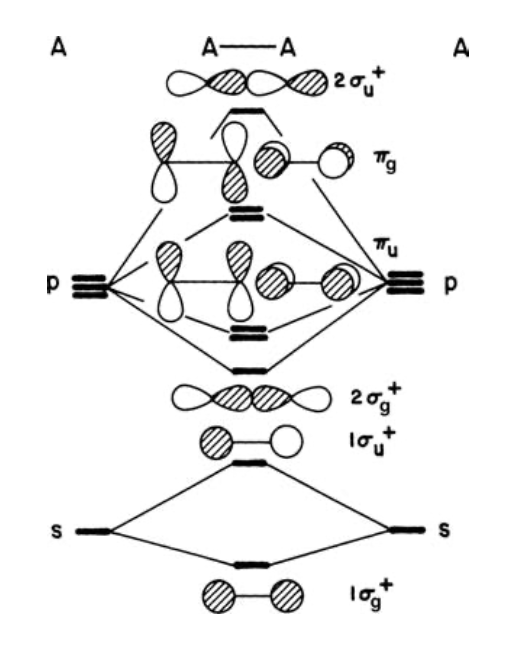
\includegraphics[width=3in]{F_A2_first_order.png}
    \caption{First order correction for a diatomic moleculars}
    \label{F:A2_first_order}
\end{figure}

Let's now consider the first order correction to the wavefunctions and the resulting 
second order change in energies. We find:
\begin{align}
    \psi_1' \approx  \psi_1^{\sigma_u} + \frac{\tilde{H}_{13} - \varepsilon_s \tilde{S}_{13}}{\varepsilon_s - \varepsilon_p} \psi_3^{\sigma_u} 
            \approx \psi_1^{\sigma_u} - |\order{t_{31}}{1}| \psi_3^{\sigma_u} \\ 
    \psi_3' \approx  \psi_3^{\sigma_u} + \frac{\tilde{H}_{13} - \varepsilon_p \tilde{S}_{13}}{\varepsilon_p - \varepsilon_s} \psi_1^{\sigma_u}
            \approx \psi_3^{\sigma_u} + |\order{t_{13}}{1}| \psi_1^{\sigma_u} \\ 
    \psi_2' \approx  \psi_2^{\sigma_g} + \frac{\tilde{H}_{24} - \varepsilon_s \tilde{S}_{24}}{\varepsilon_s - \varepsilon_p} \psi_4^{\sigma_g} 
            \approx \psi_2^{\sigma_u} + |\order{t_{42}}{1}| \psi_4^{\sigma_g} \\ 
    \psi_4' \approx  \psi_4^{\sigma_g} + \frac{\tilde{H}_{24} - \varepsilon_p \tilde{S}_{24}}{\varepsilon_p - \varepsilon_s} \psi_2^{\sigma_g} 
            \approx \psi_4^{\sigma_u} - |\order{t_{24}}{1}| \psi_2^{\sigma_g}
\end{align}
since $\tilde{S}_{24} > 0$, the higher energy orbital $\psi_4$ mix into the lower energy orbitals $\psi_2$ and vice versa. Furthermore, we note 
that since orbitals can only mix if they have the same symmetry, the resulting orbitals also have the same symmetry. With the 
corrected wavefunctions, the energy corrections up to second order can be obtained. 
The resulting orbital diagram can be plotted as in figure \ref{F:A2_second_order}. 

\begin{figure}
    \centering
    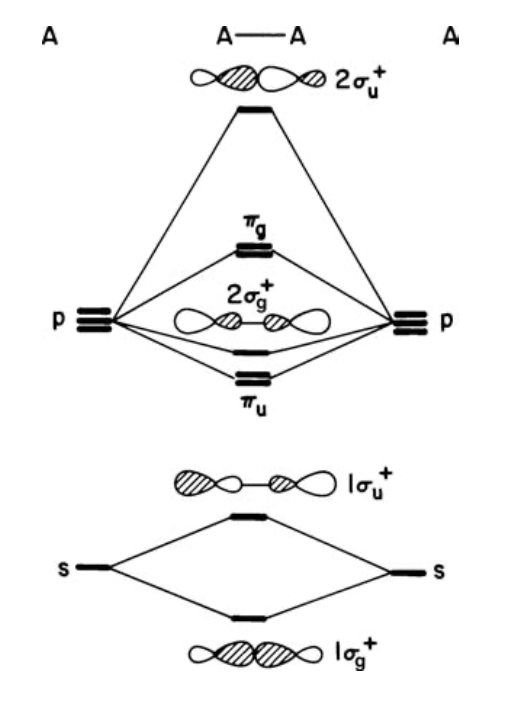
\includegraphics[width=3in]{F_A2_second_order.png}
    \caption{First order correction to the wavefunction and second order correction to the energies}
    \label{F:A2_second_order}
\end{figure}



\end{document}
